\chapter{Introducción}
Este proyecto es software libre, y está publicado con la licencia \cite{gplv3} General Public License v3.
Se puede acceder a través de GitHub en este \href{https://github.com/pablojjimenez/TFG}{enlace} puedes sentirte libre de contribuir a 
el mediante una solicitud de fusión o \textit{Pull Request}. También forma parte de los \href{https://github.com/JJ/TF-libres-UGR}{trabajos liberados}\footnote{https://github.com/JJ/TF-libres-UGR} de la UGR.

\section{Motivación} 
El tratamiento automático de la información por medio de técnicas matemáticas procesadas por un ordenador 
ha cambiado la forma en la que nos organizamos, estudiamos y obtenemos conclusiones.

Siempre he creído que la evolución en nuestra calidad de vida pasa por un
conjunto de soluciones informáticas que han de colaborar entre ellas para obtener tal propósito. 
En esta última década la recolección y almacenamiento de datos es una actividad transversal incesante 
que sin un tratamiento científico no nos aporta valor. Por distintas cuestiones personales siempre he 
estado motivado a colaborar mejorando la vida de las personas. 

Los servicios sanitarios suponen un eje vertebrador cuando hablamos de mejorar la calidad
de vida de las personas. Numerosos estudios sociológicos avalan que la sanidad es una 
preocupación incesante de los españoles. Más acentuada si cabe recientemente con la 
pandemia contra la que seguimos resistiendo.
\begin{figure}[]
	\centering	
	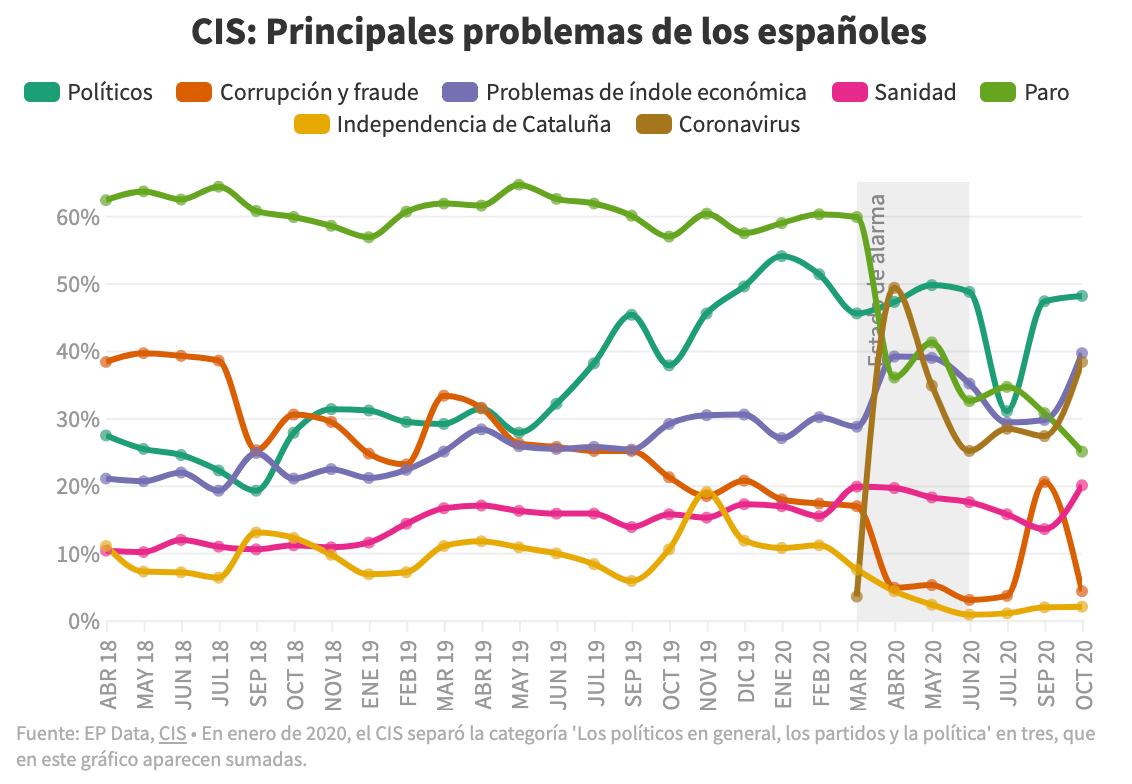
\includegraphics[scale=0.5]{doc/logos/imgs/CIS_1.png}
	\caption{ \cite{rtve-cis}  Principales problemas de los españoles según el CIS }
    \label{fig:worst_f_value}
\end{figure}

Como podemos observar en la gráfica superior; En la preocupación de los españoles la sanidad siempre se muestra con una
tendencia al alta a pesar de no estar exenta de movimientos sinusoidales. Esta tendencia solo es superada por el paro y
problemas relacionados de índole económico.

Bien es sabido que la transparencia mantiene a la población tranquila y a pesar de que estos datos
sean accesibles para la población sin un tratamiento informático y matemático de estos es como si no estuvieran. Se hace
muy difícil poder consultarlos para obtener información concreta y útil. Si ni siquiera podemos consultar datos por
variables, muy lejos estamos de poder realizar visualizaciones o tener aplicaciones que sean capaces de obtener valor de
estos datos.

\section{Usuarios}
\label{sec:usu}
una de las herramientas que nos permiten definir el alcance y las necesidades de la aplicación es la creación de
perfiles de personas ficticias, candidatos a utilizar el sistema en un futuro.

De esta forma, podemos justificar las decisiones tomadas en aras de alcanzar el objetivo por parte de los usuarios
interesados en el producto final. Vamos a tratar de crear tres personalidades lo más variopintas posibles en aras
de enfocarnos más aún en el usuario y dotar de mayor calidad el resultado final, de modo que podamos abarcar por
completo las necesidades de estos.

\rowcolors{1}{gray!20}{gray!8}
\begin{table}[H]
	\begin{center}
		\begin{tabular}{| p{\dimexpr 0.25\linewidth-2\tabcolsep} |
                   p{\dimexpr 0.8\linewidth-2\tabcolsep} |}
			\hline
			Persona 1 &  \\ \hline
			\textbf{Nombre} & Carlos \\
			\textbf{Edad} & 49 años \\
			\textbf{Formación} & Periodista \\
			\textbf{Personalidad} & \begin{itemize}
                \item Seguro de sí mismo.
                \item Motivador.
                \item Deportista.
            \end{itemize} \\
			\textbf{¿Cuál es su entorno?} & \begin{itemize}
                \item Sus amigos.
                \item Sus compañeros de trabajo.
                \item Su pareja.
            \end{itemize} \\
			\textbf{¿Qué dispositivos utiliza en su día a día?} & \begin{itemize}
                \item Un smartphone que le sirve entre otras cosas para grabar las entrevistas.
                \item Un tablet que le sirve para llevar la documentación a las entrevistas y consultar diarios.
                \item Un smartwatch.
                \item Un ordenador de sobremesa en la oficina.
            \end{itemize} \\
            \textbf{¿Cuál es su actitud hacía la tecnología?} & \begin{itemize}
                \item Atrevido.
                \item Utiliza distintos sistemas operativos.
                \item Soltura con aplicaciones ofimáticas.
                \item Soltura navegando a través de internet.
            \end{itemize} \\
            \hline
		\end{tabular}
		\caption{Usuario ficticio 1}
	\end{center}
\end{table}

\rowcolors{1}{gray!20}{gray!8}
\begin{table}[H]
	\begin{center}
		\begin{tabular}{| p{\dimexpr 0.25\linewidth-2\tabcolsep} |
                   p{\dimexpr 0.8\linewidth-2\tabcolsep} |}
			\hline
			Persona 1 &  \\ \hline
			\textbf{Nombre} & Raquel \\
			\textbf{Edad} & 30 años \\
			\textbf{Formación} & Senior frontend developer \\
			\textbf{Personalidad} & \begin{itemize}
                \item Deportista.
                \item Tímida.
                \item Lógica.
            \end{itemize} \\
			\textbf{¿Cuál es su entorno?} & \begin{itemize}
                \item Sus amigos.
                \item Su gato.
                \item Sus libros.
            \end{itemize} \\
			\textbf{¿Qué dispositivos utiliza en su día a día?} & \begin{itemize}
                \item Un portátil.
                \item Un smartphone.
            \end{itemize} \\
            \textbf{¿Cuál es su actitud hacía la tecnología?} & \begin{itemize}
                \item Perezosa.
                \item Sabe programar.
            \end{itemize} \\
            \hline
		\end{tabular}
		\caption{Usuario ficticio 2}
	\end{center}
\end{table}

\rowcolors{1}{gray!20}{gray!8}
\begin{table}[H]
	\begin{center}
		\begin{tabular}{| p{\dimexpr 0.25\linewidth-2\tabcolsep} |
                   p{\dimexpr 0.8\linewidth-2\tabcolsep} |}
			\hline
			Persona 3 &  \\ \hline
			\textbf{Nombre} & Isabel \\
			\textbf{Edad} & 45 años \\
			\textbf{Formación} & Médica de familia \\
			\textbf{Personalidad} & \begin{itemize}
                \item Aventurada.
                \item Protagonista.
            \end{itemize} \\
			\textbf{¿Cuál es su entorno?} & \begin{itemize}
                \item Su familia.
                \item Sus padres.
                \item Su trabajo.
            \end{itemize} \\
			\textbf{¿Qué dispositivos utiliza en su día a día?} & \begin{itemize}
                \item Un ordenador de sobre mesa.
                \item Un smartphone.
                \item Un iPad que comparte con su marido.
            \end{itemize} \\
            \textbf{¿Cuál es su actitud hacía la tecnología?} & \begin{itemize}
                \item Limitada.
                \item Proactiva.
            \end{itemize} \\
            \hline
		\end{tabular}
		\caption{Usuario ficticio 3}
	\end{center}
\end{table}


\section{Objetivos}
\label{sec:obj}
El objetivo principal de este proyecto es que el sistema sea capaz de darle a los usuarios la capacidad de conocer
la evolución de las causas de muerte. Las causas de muerte son clasificadas según la Clasificación Internacional
de Enfermedades y están clasificadas atendiendo a distintas variables. El sistema debe de atender a usuarios con
necesidades distintas, para identificar estas necesidades se ha utilizado la herramienta de personas ficticias,
como se ha explicado en la sección superior.